% Main document PNSAC newsletter
% Language: Latex
%

% ................................................................... %
% Preamble .......................................................... %

\documentclass[a4paper]{report}


% Use named colours (68 standard colours known to dvips)
\usepackage[usenames,dvipsnames]{color}
\usepackage{yfonts,color}

\usepackage{amssymb,amsmath}

% Note: Need to include amsmath before PNSAC, because the latter redefines the
% equation environment.
\usepackage{../PNSAC} 
% \usepackage[round]{natbib}
% To control float placement
\usepackage{stfloats}
\usepackage{float}

% for Sweave
\usepackage{listings}

% for tcltk-update
\usepackage{shortvrb}

%\usepackage{chapterbib}
\sloppy{}

% Use rotating package to typeset images in landscape mode
\usepackage{rotating}

% Using caption package and \caption* to exclude figure numbers.
\usepackage{caption}

% Using subfigure package (for side-by-side images).
\usepackage{subfigure}

% Using package for Initial drop capitals
\usepackage{lettrine}

% ................................................................... %
% Begin document .................................................... %

\begin{document}

\volume{17} % \volnumber{1}
\issue{1}
\date{August 2021} 
\titlepage

%\centerline {\Large \textit {Celebrating the 70th Anniversary of the First
%Canadian Non-Stop Transcontinental Flight}}

% Editor's notes
% ..................................................... %

% Editor's notes
\begin{article}
	% Template PNSAC newsletter - Article % Language: Latex
%

% Head



\title{Editor's Notes} 
\author{Bruce Grant}

\maketitle

\end{multicols}

While our project has been on hold, your editor still had to find some
content for the Chronicle.

%This issue of the Chronicle carries the last of four chapters in
%Richard Lodge's story of his time at Rolls-Royce. Taken together, they
%make an interesting ethnology of an extinct industrial culture. The
%whole series is accessible through our website,
%{\color{blue}\texttt{\url{http://www.projectnorthstar.ca}}} (note that
%the location of the newsletter archive will change when the new
%website goes live) starting with the April 2013 issue of the
%Chronicle.

\vspace{12pt}

Jim Riddoch came to the rescue with a story about a
successful/disastrous flight test.  We like these kinds of
stories\textemdash too small and personal to turn up in the history books, but
they do pull you into real human experiences. There will be more of these. 

%We also have another hair-raising flying story from Tim Timmins. A
%series of previous Timmins stories can be found through the same
%website, starting with the December 2010 issue
\vspace{12pt}

Your editor became a writer too, and the writer submitted a tragic
story about a French aviatice. The story was accepted by the editor in
a blatant conflict of interest.

%Motorheads among our readers should look into Ted Devey's extensive
%writings on the Rolls-Royce Merlin, starting in the December 2006
%issue.

\vspace{12pt}

And we bring you a poem by David Lambeth, an ode to the North Star
that was first published in the Chronicle of November 2005. Volunteer
Tim Timmins had found it in a hidey-hole in the aeroplane in the early
days of our restoration project.  Enjoy!

%All together, the archived issues are a valuable web resource for
%readers with an interest in aviation history or the history of Project
%North Star.



\begin{footnotesize} \raggedleft PNSAC\\
\end{footnotesize}

\begin{multicols}{2}

% End of text.

%%% Local Variables: %%% mode: latex %%% TeX-master: main_document.tex
%%% End:

 
\end{article}

\pagebreak

% President's report
%................................................. %

% Report
\begin{article}
	
% Template PNSAC newsletter - Article
% Language: Latex
%

% Head

\title{Notes from the President}
\author{Richard Lodge}

\maketitle

As we come to the end of 2013, I think of it as an interesting year
with some disappointments and important successes. I believe we end
the year in a very positive way and I look forward to 2014 with
enthusiasm and renewed optimism.

First let me get the disappointments out of the way. 2013 was our 10th
anniversary year. We had hoped to make the event an opportunity to
show off our achievements during the first 10 years and create
additional interest around the plane. Unfortunately, due to events
beyond our control, it was not possible to stage a significant event
marking the anniversary. We therefore did our usual opening of the
plane to the public on Canada Day and marked the anniversary with our
PNSAC photographer taking photographs of members as they visited the
restored cockpit.

The second disappointment is more serious. During 2013 we did not take
on any new volunteers to work on the plane. We had several good
applicants but were unable to fit any of them into the working
schedule of volunteers at the Canada Aviation \& Space Museum
(CASM). This has two downsides; the first being that we are now
becoming short of active volunteers and the second being that we are
not training any new and sometimes younger volunteers to work on
pre-jet age aircraft. It is important to pass on the skills of the
older volunteers to younger members of our Association.

Funding the restoration of the aircraft is always a challenge and is
becoming more so as the Federal government cuts back on the funds it
appropriates to the CASM and other similar institutions..

You may well ask why I feel optimistic about 2014 after referring to
disappointments and problems. In the last two months the Directors of
PNSAC met with the Director General of CASM, Stephen Quick, and
subsequently a small group of directors met again with him together
with CASM conservation staff. The outcome of these meetings has been
an excellent exchange of views, a very firm commitment by the CASM to
continue to actively support the North Star restoration and a better
understanding by both sides of the challenges we face and possible
ways forward.

As many of you already know, volunteer work on the North Star will be
suspended for approximately the first three months of 2014. This is to
enable CASM to undertake a major reorganization of the Museum exhibits
in preparation for the centenary of the start of the First World
War. During this time the CASM professional staff will be occupied
with the reorganization and will not be able to provide the necessary
supervision of restoration work. During this time, though, we plan to
update the work plan and overall budget for completing the North Star
restoration, work on fundraising initiatives and finally update our
Memorandum of Understanding with CASM.

In addition to our hands-on restoration work, the Association has a
strong social side. Bill Tate, our Vice President, and his Special
Events team have organized some memorable bus trips, the last of which
was to Montreal in October. Bill has now turned his considerable
organizational skills to further developing our quarterly Members'
Meetings. In early December we had a great morning at CASM when
Capt. Bob Pearson of the Gimli Glider fame made a presentation to 150
of our members and members of other aviation organizations we invited
to attend. Although our Vice President has retired as an airline
captain, he certainly has not retired from anything else. Watch your
emails, Facebook and Twitter for news of events Bill and his team are
planning for 2014.

\begin{footnotesize}
    \raggedleft PNSAC\\
\end{footnotesize}

% End of text.

%%% Local Variables: 
%%% mode: latex
%%% TeX-master: main_document.tex
%%% End: 

 
\end{article}

\pagebreak

% Special
% \begin{article}
% 	% Template PNSAC newsletter - Article
% Language: Latex
%

% Head

\title{PNSAC Merchandise}
%% \author{Drew Hodge}

\maketitle

%\end{multicols}

\begin{figure}[ht!]
   \vspace{2em}
   \centering
   %name of the graphic, without the path AND in EPS format:
   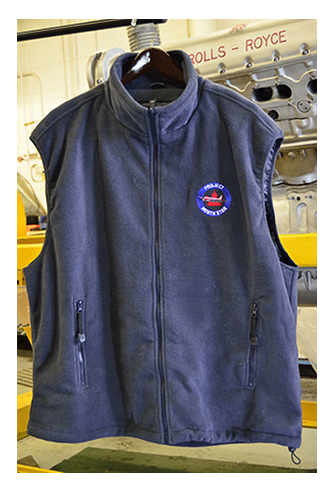
\includegraphics[scale=1.0]{fleece_YOW7578.eps}
   %caption of the figure 
   \caption*{\small \em PNSAC winter apparel}
   %label of the figure, which has to correspond to \ref{}:
   \label{fig:merchandise}
\end{figure}



The first frost warnings on the Weather Channel are reminders that
fall and winter are just around the corner. Keep warm on those frosty
fall days with a PNSAC toque and sweatshirt. We can also take
individual orders for the micro fleece vests shown in the photo on the
left, and if you're looking for early Christmas presents, how about a
coffee mug or a t-shirt?

Have a look at our Facebook page,
{\normalfont\color{blue}\texttt{\href{https://www.facebook.com/media/set/?set=a.610706705637878.1073741851.284829008225651&type=1}{PNSAC
      Merchandise}}}, to see what we're offering, and place your
orders by sending an email message to the following address
\email{pnsac.merchandise@gmail.com}.

For members in the Ottawa-Gatineau region, you can arrange to pick up
your merchandise at the Canada Aviation and Space museum any Monday or
Tuesday, between 10:00 AM and 3:00 PM. We can also ship your purchases
to you for an extra fee. Please specify museum pickup or shipping with
your order.

Merchandise is also available during our Quarterly Meetings
at CAVM.

Look forward to hearing from you.

``The Merchandise Committee''

 



\begin{footnotesize}
    \raggedleft PNSAC\\
\end{footnotesize}

%\begin{multicols}{2}

% End of text.

%%% Local Variables: 
%%% mode: latex
%%% TeX-master: main_document.tex
%%% End: 

 
% \end{article}

%\pagebreak

% Progress report ................................................... %

% Report
% \begin{article}
% 	% Template PNSAC newsletter - Article
% Language: Latex
%

% Head

\title{Project Manager's Progress Report}
\subtitle{July 2013}
\author{Bruce Gemmill}

\maketitle

Looking back on the last ten years of restoration work, we have
achieved a great deal, but much work still needs to be done.  Our
volunteer workforce has slimmed down somewhat, but those who continue
to work on the North Star have much to be proud of.

\section{Nr 2 Engine}
\label{sec:engines_2}

We reported last year that Engine Nr 2 was finished and installed on
the aircraft in April.  The spinner was repainted after it was
discovered that the paint did not stand up to the harsh outdoor
environment.  The propeller and spinner were installed on the aircraft
before it was moved outside early this year.

\section{Nr 3 Engine}
\label{sec:engines_3}

The third engine was disassembled and most of the major assemblies
were cleaned, restored and re-installed over the past year.  This
included the engine block, pistons, cylinder heads, valve train and
crankcase.  The work has gone very quickly, thanks in part to a well
organized and experienced engine shop crew, led by Garry Dupont.  A
lot of detail work has gone into some small and intricate assemblies
that no one will see once the engine is completely assembled, but that
does not mean we don't take the time to get the job done right.  The
built up engine was recently installed on the engine frame.

\begin{figure}[htbp]
   \vspace{2em}
   \centering
   %name of the graphic, without the path AND in EPS format:
   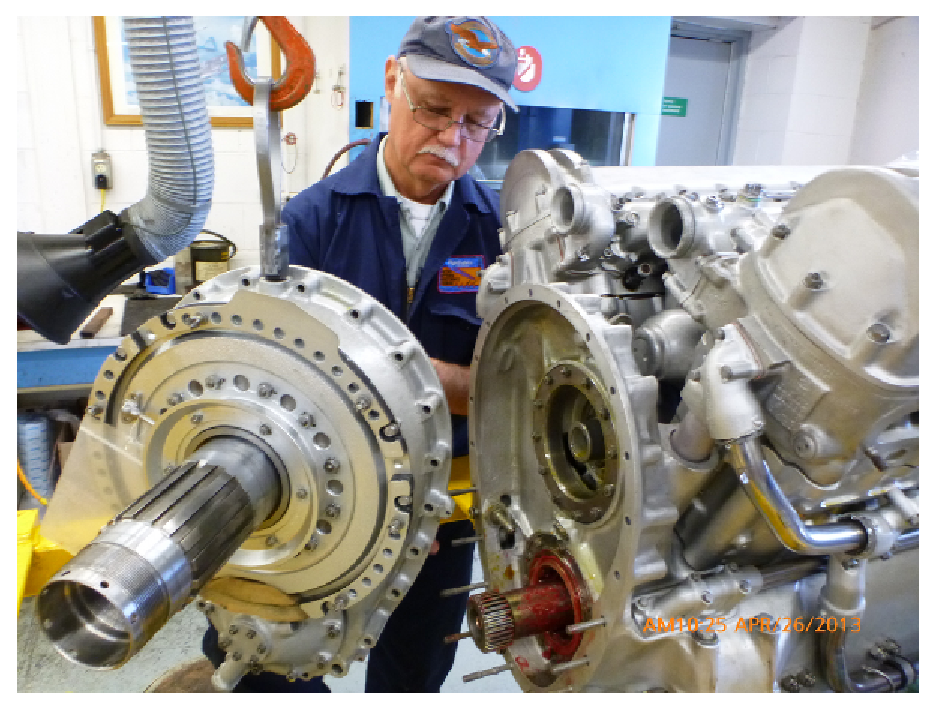
\includegraphics[scale=0.5]{engine3_reduction_gear.eps}
   %caption of the figure 
   \caption*{\small \em Garry Dupont inspecting engine nr 3's
     reduction gearbox.}
   %label of the figure, which has to correspond to \ref{}:
   \label{fig:engine3gearbox}
\end{figure}

Items still requiring restoration are the supercharger and
intercooler, and the auxiliary drive gearbox.  As always, there are
numerous pipes and hoses and fittings that also need attention.  The
engine should be completed by the end of this year.

\section{Engine Frame}
\label{engineframe}

The engine frame was completely disassembled, stripped of paint and
oil, and then repainted and the main components reassembled on the QEC
stand.  The three radiators (water, oil, and intercooler) were
thoroughly cleaned and then repainted and installed.  The cowl support
frame is currently being worked on, but some parts have been added to
the engine frame, along with the fire detectors and fire suppression
system pipes.  The large chin cowl and some of the lower cowls have
been restored.  The top and side cowls still require extensive
restoration.  This work is somewhat hampered by the small number of
volunteers available to work on these items.

\begin{figure}[htbp]
   \vspace{2em}
   \centering
   %name of the graphic, without the path AND in EPS format:
   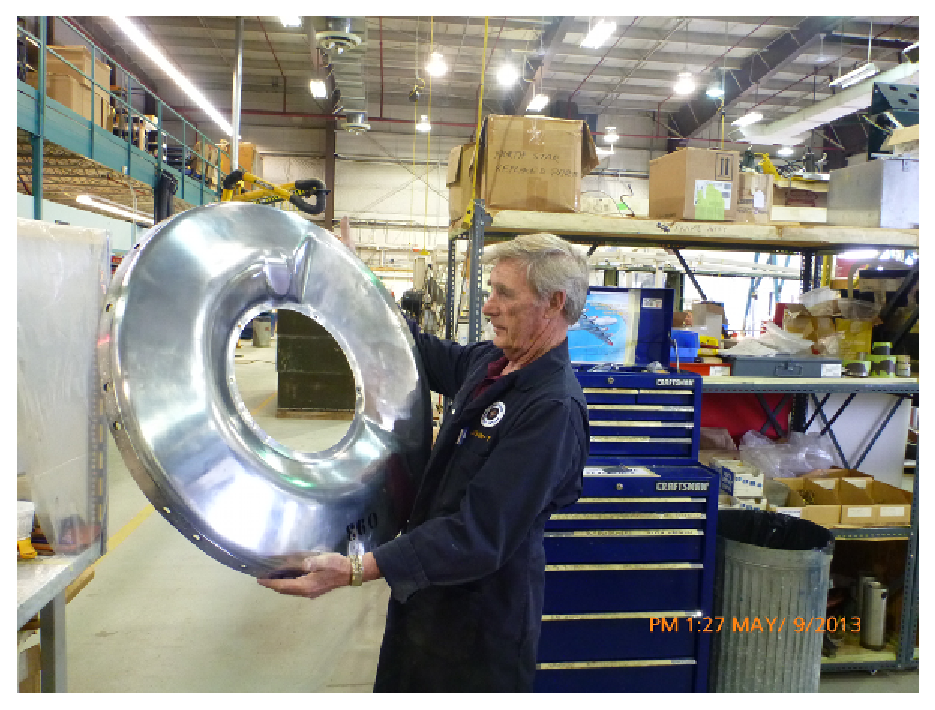
\includegraphics[scale=0.5]{engine3_prop_cowl.eps}
   %caption of the figure 
   \caption*{\small \em John Thibert with the propeller cowl for
     engine nr 3.}
   %label of the figure, which has to correspond to \ref{}:
   \label{fig:engine3propcowl}
\end{figure}


\section{Crew Lounge, Galley,  and Forward Washroom}
\label{crewlounge}

Last spring we removed the equipment from the crew lounge, galley and
forward washroom.  While the aircraft was outside these areas were
cleaned, stripped of paint, then repainted.  The flooring was removed
so the underfloor could be cleaned and primed.  There is some
corrosion damage that must be repaired before new flooring can be
installed.  Most items removed from these areas were restored over the
winter.  This included the washroom door, toilet and washroom
fittings, vanity sink and mirror, and the power inverter installed
opposite the forward washroom.  The old galley was removed and
inspected.  Due to heavy corrosion it was decided to build a
completely new galley, using the old one as a template.  Only the
original doors were retained.  The new galley is complete and will be
stored until it can be installed in the crew lounge.

The heaters had been removed from the ceiling in 2006 and fully
restored, but the air ducts, fuel lines and intake and exhaust scoops
required extensive restoration.  The air scoop was removed from the
aircraft, repaired and re-installed.  The ducts were cleaned, repaired
and new protective heat covers sewn over the old covering.  The water
tank and fittings were removed, cleaned and a new cover sewn over the
tank before installation.  New insulation was installed in the
ceiling, then most heating ducts, cables and pipes were installed.
Several fuel lines had been cut to allow removal of the Janitrol
heaters, and these need to be replaced before the heaters can be
installed.  The doors on the main electrical panel were restored and
installed.  New legends were produced to indicate the circuit breaker
and junction box connections.  These will be laminated and installed
shortly.

\section{Fuselage and Empennage}
\label{empenage}

The rear baggage compartment was cleaned and repainted.  Several floor
panels had stretched and cracked, so new panels were fabricated.  All
panels were stencilled with their respective part numbers before being
installed.  The belly compartment hatch was removed, repaired, painted
and installed.  Recently, the two battery elevators were removed, the
compartment painted, and the elevators will be repainted and installed
shortly.  Batteries were removed when the aircraft arrived at the
museum.  There has been some discussion about obtaining new
(non-functional) batteries to complete this item or work.

Most of the main fuselage was polished while inside the storage
hangar.  The underside and wings still require a lot of work.

Work is progressing on fabricating a complete set of troop seats to
fit up the interior of the main cabin, once this is restored.

\section{Planned Restoration Work--2013}
\label{sec:plannedwork}

Over the next year, we hope to have engine Nr 3 completed and engine
Nr 4 removed.  We will complete the reassembly of the crew lounge and
galley.  We then plan to work on the main cargo compartment, including
refurbishing the main heater duct and other fittings, and removing
floors to begin cleaning and repairs under the cargo floor.  We may
yet get to work on the four engine nacelles.

\section{Membership Report 2012--2013}
\label{sec:membership}

In 2012 we recorded 100 paid members and provided lifetime memberships
to two long serving volunteers and PNSAC Directors, Tim Timmins and
Jim Riddoch.

So far in 2013, we have a total of 66 new or renewed memberships.
This is slightly lower than the same time last year.  Normally, we
would expect to receive a large number of new memberships during
outside displays in the summer, but because of programming changes at
the Museum, our ability to attract new members will be greatly
reduced.

\begin{footnotesize}
  \raggedleft PNSAC\\
\end{footnotesize}

% End of text.

%%% Local Variables: 
%%% mode: latex
%%% TeX-master: main_document.tex
%%% End: 

 
% \end{article}

\pagebreak

% Member interview ................................................... %

% Report
\begin{article}
    % Template PNSAC newsletter - Article
% Language: Latex
%

% Head

\title{Our Members}
\author{Interview with Jm Riddoch}

\maketitle

\end{multicols}

\begin{quotation}
	\textit{Jim Riddoch is one of the earliest and longest serving members of the
Association. He has made a significant contribution to the operations of the
Association including working on the aircraft as well as being an officer and
member of the board of directors. Although officially retired from formal
positions in the organization, he can still be counted on to help out when
needed.}
\end{quotation}

\begin{multicols}{2}

1.\textit{What is your background in aviation?}

I started with English Electric Aviation Company in 1956 as an
apprentice technician eventually being assigned to the Mechanical
Engineering Department as a fuel systems technician. I remained there
for 5 years until I was 28 years old and married with a daughter. After
immigrating to Canada in March 1966 I joined DeHavilland Spar Division
in Malton and then moved to Montreal with Jarry Hydraulics as a
development engineer. I remained there for 2 years working chiefly on
development proposals for the wing sweep actuators for F111 aircraft
and Boeing's proposed supersonic Concorde.

In 1968 I joined Air Canada as a junior engineer in the Mechanical
Systems Department and assigned as a landing gear technologist until I
achieved Professional Engineer status in 1974. I then moved around
several other departments in engineering and maintenance until I was
promoted to Superintendent of DC 9 maintenance. In that capacity I was
involved in the accident investigation into the loss of one aircraft at
Cincinnati.

I eventually returned to engineering as Director of Interior Systems and
Equipment to supervise extensive fleet modifications and new aircraft
acquisitions. I remained in that position until I retired in 1990.
Following a short stint with First Air I was asked to join a newly formed
Canadian Aviation Maintenance Council to standardize aircraft
maintenance trades basic training. I was hired as the Accreditation
Manager to approve various training establishments including schools,
companies and military programs, I eventually also took on the job of
Registration Manager to accept qualified trade technicians.

2. \textit{How long have you been involved with Project North Star and how and why did you get involved?}

Following my retirement from the Canadian Aviation Maintenance
Council in 2003 I was approached by Robert Holmgren to participate in
a voluntary program to help restore an the Canadair North Star aircraft
parked outside at the Canada Aviation Museum. Along with Tim
Timmins and a few others we formed a steering committee to approach
the Museum about forming a voluntary work force to assist the museum
staff to restore the aircraft. At first we met with opposition from some
staff members who felt their jobs were being compromised and possible
staff reductions. Slowly we were approved by the Museum staff with
limited supervision and controlled access and work direction. I was
assigned by the Project North Star Association as Chief Engineer of the
project although all work was controlled and supervised by the
Museum's staff manager.

%\begin{figure}[htbp]
%   \vspace{2em}
%   \centering
%   %name of the graphic, without the path AND in EPS format:
%   \includegraphics[scale=0.5]{fwd_cockpit_complete.eps}
%   %caption of the figure 
%   \caption*{\small \em Forward cockpit -- complete.}
%   %label of the figure, which has to correspond to \ref{}:
%   \label{fig:fwd_cockpit_complete}
%\end{figure}

3. \textit{What has been the history of your involvement to date?}

I worked on the Project for 10 years starting in 2003 both as a "hands
on" volunteer as well as a member of the board of directors and officer
of the Association. Generally I put in at least two days per week and
sometimes more. 

%\begin{figure}[htbp]
%	\vspace{2em}
%	\centering
%	%name of the graphic, without the path AND in EPS format:
%	\includegraphics[scale=0.9]{resources/PNS2008-10-26_23-31-42.png}
%	%caption of the figure 
%	\caption*{\small \em Propeller assembly.}
%	%label of the figure, which has to correspond to \ref{}:
%	\label{fig:propeller}
%\end{figure}

%\begin{figure}[htbp]
%	\vspace{2em}
%	\centering
%	%name of the graphic, without the path AND in EPS format:
%	\includegraphics[scale=1.3]{resources/NorthStarCockpitDec2011.png}
%	%caption of the figure 
%	\caption*{\small \em Forward cockpit -- complete.}
%	%label of the figure, which has to correspond to \ref{}:
%	\label{fig:fwd_cockpit_complete}
%\end{figure}

4. \textit{What has been the highlight of your involvement?}

The chief highlights have been the high level of workmanship of the
volunteers and displaying the aircraft to the public and interested
persons.

%\begin{figure}[htbp]
%   \vspace{2em}
%   \centering
%   %name of the graphic, without the path AND in EPS format:
%   \includegraphics[scale=0.75]{resources/NavigatorRack.png}
%   %caption of the figure 
%   \caption*{\small \em Navigator rack.}
%   %label of the figure, which has to correspond to \ref{}:
%   \label{fig:nav-radio-rack}
%\end{figure}

5. \textit{What has been the most challenging part of your involvement?}

Keeping the Museum staff and management on side with our goals
and objectives and recruiting enough new volunteers to keep the
project going.

\begin{footnotesize}
    \raggedleft PNSAC\\
\end{footnotesize}



% End of text.

%%% Local Variables: 
%%% mode: latex
%%% TeX-master: main_document.tex
%%% End: 

 
\end{article}

%\pagebreak

% Features
% ........................................................... %

% Feature article

\begin{article}
	% Template PNSAC newsletter - Article
% Language: Latex
%

% Head

\title{APS 42 Radar -- Another Piece of the North Star Puzzle}

%\author{Based on Bruce Gemmill's notes; reviewed by Garry Dupont, and with editing assistance from Richard Lodge}

\maketitle

% \paragraph*{Engine 3}

\textit{The article below was written by our members John Makadi and Chris McGuffin. Chris and John played key roles in the acquisition of the APS 42 Radar for the North Star aircraft. In 2019 John was approached by R\'{e}jean Demers, CASM's project manager for the North Star restoration to see if he could locate the radar unit which was missing from the aircraft as explained below. John was successful and as a result in 2001  R\'{e}j asked Chris if  our association  could arrange for the acquisition of the unit. John and Chris coordinated its acquisition and what follows is a very fascinating story about what may be the only unit of its kind still in existence. The authors have been very modest about their contributions in dealing with a very challenging process made more difficult by the pandemic Covid-19.}

The North Star was the RCAF’s first strategic lift platform. It was dispatched across the country, and bridged the Atlantic and Pacific in service to Canada. In the late 1950s, the RCAF began upgrading the fleet with the addition of the APS-42 military navigation/weather radar. This radar was still sensitive equipment in 1966 when North Star 17515 was donated to the Canada Aviation and Space Museum. The radar was stripped out of the airframe along with the radios and other sensitive equipment.

Project North Star is frequently described as an effort to return 17515 to the condition she was in on her last day of service with the RCAF. The hunt was on. In 2019 Project North Star Association of Canada began searching for an APS-42 radar. Initial results were discouraging. US aviation museums with USAF aircraft had no components to offer. Further research of US military logistics documents revealed that US Department of Defense disposal instructions for APS-42 radar was to “Destroy” them due to their sensitive nature at the time.

\begin{figure}[H]
   \vspace{2em}
   \centering
   %name of the graphic, without the path AND in EPS format:
   \includegraphics[scale=0.45]{radar_the_unit.png}
   %caption of the figure 
   \caption*{\small \em Radar -- The Unit.}
   %label of the figure, which has to correspond to \ref{}:
   \label{fig:img1}
\end{figure}

We were disheartened by that discovery but certainly not defeated. Over the years, PNSAC volunteers have been resourceful about rescuing parts and assemblies. The search continued. In the spring of 2021, while continuing on-line research John stumbled across an eBay listing for an APS-42 transmitter out of Cross Timbers, Missouri (Ozarks). The seller, a military communications enthusiast, acquired the radar in a lot purchase of US Government surplus equipment. After negotiating an acceptable price for the radar, we just needed to get it to CASM.

\begin{figure}[H]
    \vspace{2em}
    \centering
    %name of the graphic, without the path AND in EPS format:
    \includegraphics[scale=0.5]{radar_the_aps_42.png}
    %caption of the figure 
    \caption*{\small \em Radar -- The APS-42.}
    %label of the figure, which has to correspond to \ref{}:
    \label{fig:img2}
 \end{figure}
 
Shipping freight is usually pretty straight forward. In the summer of 2021, there were “unusual” circumstances. Transportation was a bottle neck to many industries and costs rose across the carriers. We were unable to find a freight company willing to collect the radar in the seller’s remote location. Our seller was willing to deliver to Springfield, Missouri (for a fee) but would not provide a crate. Furthermore, the freight companies that offered custom crating services were prohibitively high. Then we made contact with the “Air and Military Museum of the Ozarks” (AMMO) – a small volunteer-based museum in Springfield. The volunteers at AMMO were sympathetic to our cause and enthusiastic to help. They agreed to receive our radar from the seller, build a custom crate and transfer it to the freight carrier. We were grateful to pay them a small honorarium which wasn’t much more than the cost of lumber for the crate. This was a wonderful example of museums cooperating across borders to preserve aviation heritage. AMMO ended up hosting the crated radar for several weeks. The hurdles of NAFTA attestations and the export of US military technology took additional bureaucratic kung-fu but the radar arrived safely in Ottawa on 10 June, 2021.

 \begin{figure}[H]
    \vspace{2em}
    \centering
    %name of the graphic, without the path AND in EPS format:
    \includegraphics[scale=0.5]{radar_opening_the_unit.png}
    %caption of the figure 
    \caption*{\small \em Radar -- Opening the Unit.}
    %label of the figure, which has to correspond to \ref{}:
    \label{fig:img3}
 \end{figure}

After 17 months of social distancing, Project North Star volunteers and CASM staff gathered in the parking lot to celebrate the arrival of a missing radar. Customs seals were removed and a wood crate was opened to reveal our beautifully preserved APS-42. We look forward to seeing this new artifact in the nose wheel well of 17515.

% \begin{figure}[H]
%    \vspace{2em}
%    \centering
%    %name of the graphic, without the path AND in EPS format:
%    \includegraphics[scale=0.5]{four-merlins-1.png}
%    %caption of the figure 
%    \caption*{\small \em North Star being moved inside hangar 11 August 2005 .}
%    %label of the figure, which has to correspond to \ref{}:
%    \label{fig:tim}
% \end{figure}



 

% \begin{figure}[htbp]
%    \vspace{2em}
%    \centering
%    %name of the graphic, without the path AND in EPS format:
%    \includegraphics[scale=0.5]{four-merlins-2.png}
%    %caption of the figure 
%    \caption*{\small \em  Mike Hope and Bruce Gemmill assembled Prop 1ready to
% install on Engine 1 October 26, 2008.}
%    %label of the figure, which has to correspond to \ref{}:
%    \label{fig:tim}
% \end{figure}



% \begin{figure}[htbp]
%    \vspace{2em}
%    \centering
%    %name of the graphic, without the path AND in EPS format:
%    \includegraphics[scale=0.55]{four-merlins-3.png}
%    %caption of the figure 
%    \caption*{\small \em Engine 1 assembled in the Conservation shop Feb 2,
% 2010.}
%    %label of the figure, which has to correspond to \ref{}:
%    \label{fig:tim}
% \end{figure}

% \begin{figure}[htbp]
%    \vspace{2em}
%    \centering
%    %name of the graphic, without the path AND in EPS format:
%    \includegraphics[scale=0.55]{four-merlins-4.png}
%    %caption of the figure 
%    \caption*{\small \em Firewall ready, auxiliary gearbox installed Jan 7,
% 2010.}
%    %label of the figure, which has to correspond to \ref{}:
%    \label{fig:tim}
% \end{figure}



% \begin{figure}[htbp]
%    \vspace{2em}
%    \centering
%    %name of the graphic, without the path AND in EPS format:
%    \includegraphics[scale=0.55]{four-merlins-5.png}
%    %caption of the figure 
%    \caption*{\small \em Engine 1 complete at the Restoration Shop Feb 9, 2010
% .}
%    %label of the figure, which has to correspond to \ref{}:
%    \label{fig:tim}
% \end{figure}

% \begin{figure}[htbp]
%    \vspace{2em}
%    \centering
%    %name of the graphic, without the path AND in EPS format:
%    \includegraphics[scale=0.45]{four-merlins-6.png}
%    %caption of the figure 
%    \caption*{\small \em Engine 1 installed Feb 24, 2010. Shown top left to
% bottom right, engine
% supervisor Ted Devey,  Bill Tate, Ron Lemieux, Giuseppe Zanetti, John Corby,
% Garnet Chapman, Volunteer Project Manager Jim Riddoch, John Tasseron, Bruce
% Gemmill, Museum Project Coordinator Mike Irvin, Charles Baril, and then
% Association President Tim Timmins.}
%    %label of the figure, which has to correspond to \ref{}:
%    \label{fig:tim}
% \end{figure}



% \paragraph*{Engine 2}\



% \begin{figure}[htbp]
%    \vspace{2em}
%    \centering
%    %name of the graphic, without the path AND in EPS format:
%    \includegraphics[scale=0.5]{four-merlins-8.png}
%    %caption of the figure 
%    \caption*{\small \em Engine 2 with cowl panels removed, April 6, 2010.}
%    %label of the figure, which has to correspond to \ref{}:
%    \label{fig:tim}
% \end{figure}



% \begin{figure}[htbp]
%    \vspace{2em}
%    \centering
%    %name of the graphic, without the path AND in EPS format:
%    \includegraphics[scale=0.5]{four-merlins-9.png}
%    %caption of the figure 
%    \caption*{\small \em Engine 2 removed April 14, 2010.}
%    %label of the figure, which has to correspond to \ref{}:
%    \label{fig:tim}
% \end{figure}



% \begin{figure}[htbp]
%    \vspace{2em}
%    \centering
%    %name of the graphic, without the path AND in EPS format:
%    \includegraphics[scale=0.5]{four-merlins-10.png}
%    %caption of the figure 
%    \caption*{\small \em Stan Rideout working to reassemble Engine 2 in engine
% shop, Oct 7, 2010.}
%    %label of the figure, which has to correspond to \ref{}:
%    \label{fig:tim}
% \end{figure}



% \begin{figure}[htbp]
%    \vspace{2em}
%    \centering
%    %name of the graphic, without the path AND in EPS format:
%    \includegraphics[scale=0.5]{four-merlins-11.png}
%    %caption of the figure 
%    \caption*{\small \em Austin (Tim) Timmins.}
%    %label of the figure, which has to correspond to \ref{}:
%    \label{fig:tim}
% \end{figure}



% \begin{figure}[htbp]
%    \vspace{2em}
%    \centering
%    %name of the graphic, without the path AND in EPS format:
%    \includegraphics[scale=0.5]{four-merlins-12.png}
%    %caption of the figure 
%    \caption*{\small \em Jim Riddoch and Bill Tate fill the radiators with
% inhibiting oil.}
%    %label of the figure, which has to correspond to \ref{}:
%    \label{fig:tim}
% \end{figure}


% \begin{figure}[htbp]
%    \vspace{2em}
%    \centering
%    %name of the graphic, without the path AND in EPS format:
%    \includegraphics[scale=0.7]{four-merlins-13.png}
%    %caption of the figure 
%    \caption*{\small \em Engine 2 on rotating assembly stand.}
%    %label of the figure, which has to correspond to \ref{}:
%    \label{fig:tim}
% \end{figure}

 

% \begin{figure}[htbp]
%    \vspace{2em}
%    \centering
%    %name of the graphic, without the path AND in EPS format:
%    \includegraphics[scale=0.45]{four-merlins-14.png}
%    %caption of the figure 
%    \caption*{\small \em  Engine Nr 2 being re-assembled in the engine shop.}
%    %label of the figure, which has to correspond to \ref{}:
%    \label{fig:tim}
% \end{figure}



% \begin{figure}[htbp]
%    \vspace{2em}
%    \centering
%    %name of the graphic, without the path AND in EPS format:
%    \includegraphics[scale=0.5]{four-merlins-15.png}
%    %caption of the figure 
%   % \caption*{\small \em .}
%    %label of the figure, which has to correspond to \ref{}:
%    \label{fig:tim}
% \end{figure}



\begin{footnotesize}
    \raggedleft PNSAC\\
\end{footnotesize}


% End of text.

%%% Local Variables: 
%%% mode: latex
%%% TeX-master: main_document.tex
%%% End: 

 
\end{article}

\pagebreak

% Feature article
% \begin{article}                 
% 	% Template PNSAC newsletter - Article % Language: Latex
%

% Head

\title{The Civil Merlin} 
\author{Dr. Jakob Whitfield}
\maketitle

\textit{The following article is an extract from a larger piece which appeared
in the July 2017 edition of Aeroplane magazine under the heading
"Rolls-Royce Merlin."  We wish to thank Allan Bowes for bringing it to
our attention. This article is republished with the kind permission of
the publishers of the magazine and the author Dr. Jakob Whitfield.}\\


The earliest Merlins to operate in a civil mode were the Merlin T24
series, developed in 1944. These were single-stage twin-speed units
similar to the Merlin 24s fitted to the RAF's Lancasters, but were
modified to improve service life, and were fitted to Transport
Command's Avro Yorks. Long-range transport operation entailed running
at relatively low cruise powers for long periods---under these
conditions the lower cylinder head temperatures caused deposits of lead
oxide from the fuel, resulting in excessive spark plug fouling. To
counter this, the Merlin T24/4 incorporated a charge heater to increase
the inlet temperature. Post-war, the Merlin 500 series essentially
comprised civil and export versions of the T24, incorporating its
modifications, though only the Merlin 501 included a charge heater.

\begin{figure}[httb]
   \vspace{2em}
   \centering
   \includegraphics [scale=0.5]{merlin-1-feb-2020.jpg}
   \caption*{\small \em Rolls-Royce Merlin Engine}
   \label{fig:wall-two}
\end{figure}

The 600 and 700-series engines were two-speed two-stage engines, based
on the military 100-series. They were fitted with the so-called
'transport heads and banks', strengthened for greater reliability. Most
marks had some form of variable intercooling to allow for charge
heating to reduce plug fouling under cruise conditions. Initially the
system was plagued by coolant leaks, but as experience showed that zero
intercooling at cruise allowed enough charge heating to reduce leading,
a simple stop valve was fitted to the system. This allowed full
intercooling for take-off and climb, which could then be turned off for
cruise.

Civil Merlins were fitted to Avro Lancastrians, Yorks and Tudors, but
their flagship role was on the Canadair DC-4M North Star, a Douglas
DC-4-derived design intended for Trans-Canada Air Lines (TCA). The
North Stars used a modified Universal Power Plant installation, as the
DC-4's nacelle bulkheads were slightly larger than the SBAC standard.
In practice it turned out the Merlins were not ideally suited for use
in civil operations: though the North Stars flew higher and faster than
DC-4s, their time between engine overhauls was around 850 hours,
roughly a third of that of commercial US radial engines. The engines
also produced a lot of cabin noise, though this was alleviated somewhat
by revised 'cross-over' exhausts that ducted the cabin-side stacks
outboard, developed first by TCA and then by Rolls-Royce themselves.

\begin{figure}[httb]
   \vspace{2em}
   \centering
   \includegraphics[scale=0.5]{nstar-tca-feb-2020.jpg}
   \caption*{\small \em TCA Canadair DC-4M North Star}
   \label{fig:wall-two}
\end{figure}

The extra running costs were mostly borne by Rolls-Royce. When TCA's
managing director expressed dissatisfaction with the Merlin's
commercial performance, Hives asked what a reasonable level of
maintenance cost would be. Being told \$4 per engine hour, he agreed to
service the fleet's engines for this amount. This early form of 'power
by the hour' was initially expensive for Rolls-Royce, but by the end of
the Merlin's life the company had learned enough to supposedly make a
small profit at this level.

What was undoubtedly true was that Rolls-Royce learned a great deal
about the harsh realities of commercial operation in a short time.
Hives is supposed to have said to TCA, "We didn't know the Merlin until
you started operating it!" In the longer term, this paid off,
TCA---later Air Canada---selecting Rolls--Royce engines for its future
fleet: Darts in Viscounts, Tynes in Vanguards, Conways in DC-8s, and
RB211s in TriStars.


\begin{footnotesize} \raggedleft PNSAC\\
\end{footnotesize}

% End of text.

%%% Local Variables: %%% mode: latex %%% TeX-master: main_document.tex
%%% End:

 
% \end{article}

\pagebreak

% Feature article
% \begin{article}
% 	% Template PNSAC newsletter - Article
% Language: Latex
%

% Head

\title{Troop Seats and Extras}
\author{Nelson Smith}

\maketitle

\section{Troop Seats}
\label{troopseats}

Seat back assemblies are completed for the troop seats. Thirty eight
units were produced. The assembling of the backs to the platforms to
produce triple and quad seats will be the next step. This will be done
over the winter.

\begin{figure}[htbp]
   \vspace{2em}
   \centering
   %name of the graphic, without the path AND in EPS format:
   \includegraphics[scale=0.5]{troopseats.eps}
   %caption of the figure 
   \caption*{\small \em New troop seats.}
   %label of the figure, which has to correspond to \ref{}:
   \label{fig:troopseats}
\end{figure}

The prototype is progressing well. As previously stated, measurements
are a rarity with these projects and sometimes it takes longer to
figure out a plan than to do the job. A guesstimate for completion:
early December.


\section{Other Projects}
\label{otherporjects}

Proctective covers for the probes which protrude under the belly of
the North Star were made and installed. The foam pads previously
installed had done their time.

The First Officer's protective seat covers have been manufactured and
installed. This addition was required to shield the seat covers from
UV rays, dust and stains. Similar covers will be made for the
Captain's chair during the winter months.

\begin{footnotesize}
    \raggedleft PNSAC\\
\end{footnotesize}

% End of text.

%%% Local Variables: 
%%% mode: latex
%%% TeX-master: main_document.tex
%%% End: 

 
% \end{article}

%\pagebreak


% Recent events ...................................................... %

%\begin{article}                 
%	

% Template PNSAC newsletter
% Language: Latex


\title{Canada Day 2016}
\author{Bill Tate}

\maketitle

Canada Day at the Museum always provides us with an opportunity to show off what
PNSAC is and does; and July 1, 2016 was no exception. Fortunately the weather
was ideal for most of the day. Our volunteers partially set up our display on
June 30th and the balance was done early in the morning of July1st.

Our display, unlike the picture shown below from 2011, was limited by the nose
section being shrink wrapped in plastic to prevent water damage. Consequently,
we unable to show off the cockpit because of lighting issues and ventilation.
This could have been rectified with additional fans and lights but with
restoration work being done on the main cabin floor, visits were limited to
viewing from just inside the aircraft rear cargo door.

Although not widely known we are also limited by the number of people. we can
have inside the aircraft at any one time. There is a reason for this as an empty
aircraft "generally" has the centre of gravity in the aft range limit and with
the engine \#4 off the aircraft this becomes even more pronounced. For this
reason sand bags have been placed in the forward cargo hold to help keep the
centre of gravity as far forward as possible. This limits us to having a maximum
of four adults or a family with children in at one time and yes we have to
include our volunteers so that we do not exceed the equivalent of six adults.


%\begin{figure}[htbp]
%   \vspace{2em}
%   \centering
%   %name of the graphic, without the path AND in EPS format:
%   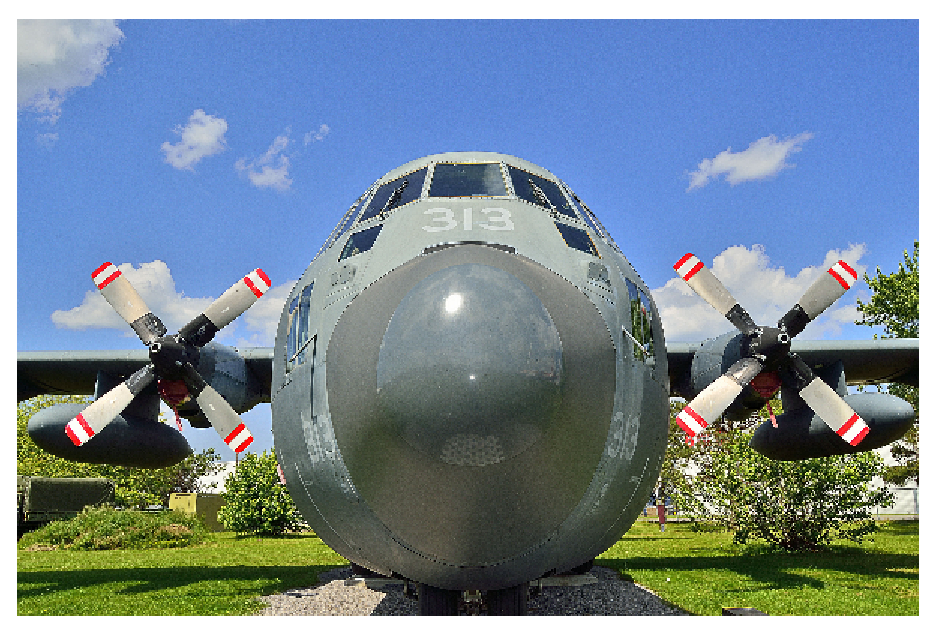
\includegraphics[scale=0.5]{trenton2013-herc.eps}
%   %caption of the figure 
%   \caption*{\small \em National Air Force Museum -- Hercules.}
%   %label of the figure, which has to correspond to \ref{}:
%   \label{fig:herc}
%\end{figure}


\end{multicols}

\begin{figure*}[ht!]
   \vspace{2em}
   \centering
   %name of the graphic, without the path AND in EPS format:
   \includegraphics[scale=0.75]{canada-day-2016}
   %caption of the figure 
   \caption*{\small \em Canada Day 2016.}
   %label of the figure, which has to correspond to \ref{}:
   \label{fig:canadaday}
\end{figure*}

\begin{multicols}{2}

The weather forecast that day was for thunder storm activity and as the day
progressed the skies darkened. For the safety of our volunteers and public we
shut down our display earlier than normal because as the wind increased we had
some of our story boards blown over by gusts of wind. As an aside, airports with
"Thor Guard" cease ramp operations when a thunderstorm is within 6 nautical
miles.

Our display attracted many visitors and there was a continuous line of people
waiting patiently for their turn to climb the steps and view the aircraft
interior. As in previous years we also took the covers off engine \#2 so we could
show an engine to our visitors after it had been fully restored.

I would like to thank all our volunteers who made Canada Day such a success and
to mention the very demanding work performed by Bruce Grant and Jim Riddoch who
handled crowd control, and John Thibert and Charles Baril who spent several
hours in the hot interior of the North Star talking to our visitors about the
work that went on inside the airplane.

Any suggestions to improve our display, who we are and what we do would be most
appreciated. Please send to Bill Tate.

\begin{footnotesize}
    \raggedleft PNSAC\\
\end{footnotesize}

%%% Local Variables: 
%%% mode: latex
%%% TeX-master: main_document.tex
%%% End: 

%\end{article}

%\pagebreak


%\vspace{35 mm}

% \begin{article}                 
% 	

% Template PNSAC newsletter
% Language: Latex


\title{Canada Day 2016}
\author{Bill Tate}

\maketitle

Canada Day at the Museum always provides us with an opportunity to show off what
PNSAC is and does; and July 1, 2016 was no exception. Fortunately the weather
was ideal for most of the day. Our volunteers partially set up our display on
June 30th and the balance was done early in the morning of July1st.

Our display, unlike the picture shown below from 2011, was limited by the nose
section being shrink wrapped in plastic to prevent water damage. Consequently,
we unable to show off the cockpit because of lighting issues and ventilation.
This could have been rectified with additional fans and lights but with
restoration work being done on the main cabin floor, visits were limited to
viewing from just inside the aircraft rear cargo door.

Although not widely known we are also limited by the number of people. we can
have inside the aircraft at any one time. There is a reason for this as an empty
aircraft "generally" has the centre of gravity in the aft range limit and with
the engine \#4 off the aircraft this becomes even more pronounced. For this
reason sand bags have been placed in the forward cargo hold to help keep the
centre of gravity as far forward as possible. This limits us to having a maximum
of four adults or a family with children in at one time and yes we have to
include our volunteers so that we do not exceed the equivalent of six adults.


%\begin{figure}[htbp]
%   \vspace{2em}
%   \centering
%   %name of the graphic, without the path AND in EPS format:
%   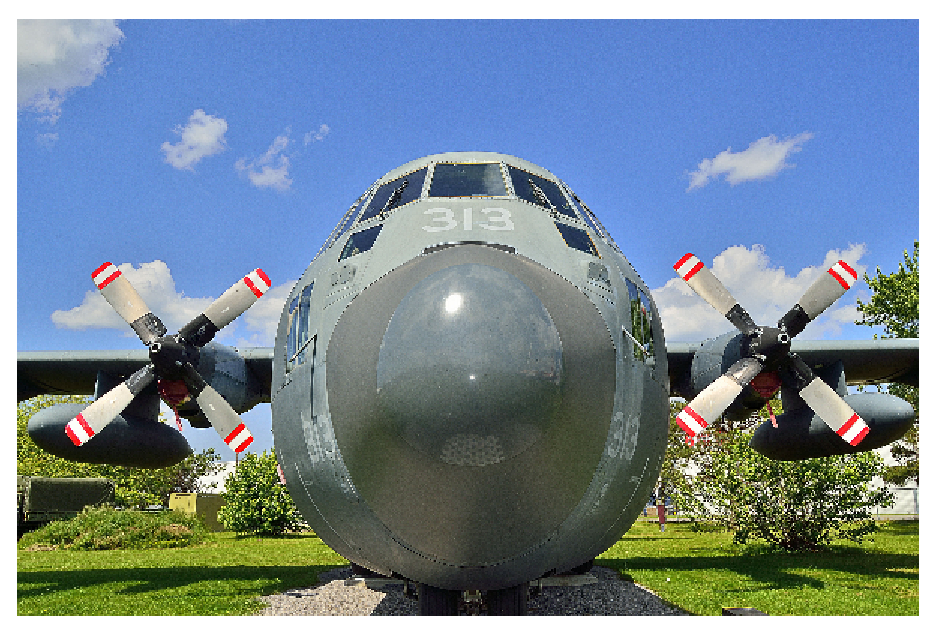
\includegraphics[scale=0.5]{trenton2013-herc.eps}
%   %caption of the figure 
%   \caption*{\small \em National Air Force Museum -- Hercules.}
%   %label of the figure, which has to correspond to \ref{}:
%   \label{fig:herc}
%\end{figure}


\end{multicols}

\begin{figure*}[ht!]
   \vspace{2em}
   \centering
   %name of the graphic, without the path AND in EPS format:
   \includegraphics[scale=0.75]{canada-day-2016}
   %caption of the figure 
   \caption*{\small \em Canada Day 2016.}
   %label of the figure, which has to correspond to \ref{}:
   \label{fig:canadaday}
\end{figure*}

\begin{multicols}{2}

The weather forecast that day was for thunder storm activity and as the day
progressed the skies darkened. For the safety of our volunteers and public we
shut down our display earlier than normal because as the wind increased we had
some of our story boards blown over by gusts of wind. As an aside, airports with
"Thor Guard" cease ramp operations when a thunderstorm is within 6 nautical
miles.

Our display attracted many visitors and there was a continuous line of people
waiting patiently for their turn to climb the steps and view the aircraft
interior. As in previous years we also took the covers off engine \#2 so we could
show an engine to our visitors after it had been fully restored.

I would like to thank all our volunteers who made Canada Day such a success and
to mention the very demanding work performed by Bruce Grant and Jim Riddoch who
handled crowd control, and John Thibert and Charles Baril who spent several
hours in the hot interior of the North Star talking to our visitors about the
work that went on inside the airplane.

Any suggestions to improve our display, who we are and what we do would be most
appreciated. Please send to Bill Tate.

\begin{footnotesize}
    \raggedleft PNSAC\\
\end{footnotesize}

%%% Local Variables: 
%%% mode: latex
%%% TeX-master: main_document.tex
%%% End: 

% \end{article}

\pagebreak

% Special article 
%\begin{article}
%	


% Template PNSAC newsletter
% Language: Latex


\title{Quarterly Meeting Report}
\author{Drew Hodge}

\maketitle

On Saturday 7th December 2013, Project North Star Association of
Canada (PNSAC) held a quarterly meeting in the auditorium of the
Canadian Aviation and Space Museum (CASM) in Ottawa. It was a
memorable meeting with over 200 people in attendance. Those in the
audience that day were able to hear the story of the Gimli Glider told
in person by Captain (retd.) Robert (Bob) Pearson, the pilot of Air
Canada Boeing 767-200, fin number 604, when it made an unscheduled
stop at Gimli Manitoba, thirty years ago.

The meeting started with an introduction by Bill Tate, Project North
Star's Vice President.  Bill began by welcoming the audience, which,
as well as PNSAC volunteers, included members of Vintage Wings of
Canada, Ottawa Airport Watch, the Canadian Aviation Historical
Society, the College of Professional Pilots of Canada, CASM volunteers
and staff, Air Canada and WestJet pilots, and visitors from the
general public, one of whom had travelled to Ottawa from Vancouver for
the meeting. After describing the goals of Project North Star and
asking PNSAC volunteers to stand and be recognized, Bill invited the
audience to visit the world class exhibits in the Museum after the
meeting.

Bill's acquaintance with Bob Pearson goes back thirty-five years, when
Bill was Captain Pearson's Second Officer on Boeing 727s based in
Montreal. His duties in the cockpit back then gave Bill ample
opportunities to watch Captain Pearson at work. Bill described Captain
Pearson as a "highly professional pilot" who, "wearing his command
lightly", demonstrated "highly polished interpersonal skills and a
delightful sense of humour".  He then invited Captain Pearson to tell
the story of flying unscheduled into Gimli.

Captain Pearson spoke for a little over an hour with no notes and with
reference to a few appropriate slides.  He described eloquently how,
because of errors in the conversion of metric measurements, his Boeing
767-200 ran out of fuel and lost both engines over Manitoba on the way
from Ottawa to Edmonton. The full story is well documented in the book
"Freefall: From 41,000 feet to zero - a true story, William and
Marilyn Hoffer, Simon \& Schuster, 1989", but to hear it told in
person by the pilot in command that Saturday, 23rd July, 1983, was a
rare privilege.

\begin{figure}[htbp]
   \vspace{2em}
   \centering
   %name of the graphic, without the path AND in EPS format:
   \includegraphics[scale=0.9]{Pearson004.eps}
   %caption of the figure 
   \caption*{\small \em Captain (retd.) Robert Pearson.}
   %label of the figure, which has to correspond to \ref{}:
   \label{fig:pearson004}
\end{figure}

The port engine stopped first at 41,000 feet prompting the decision to
divert to Winnipeg.  At 28,000 feet the starboard engine ran down too,
and Maurice Quintal, Captain Pearson's First Officer, made
calculations that showed they couldn't reach Winnipeg.  Quintal
advised Captain Pearson to try for the nearest runway on the former
RCAF aerodrome at Gimili, twelve miles away.  Some eight or ten
minutes after losing the first engine, Captain Pearson side-slipped
the big Boeing down to an old runway that was being used as a racing
track by members of the Winnipeg Sports Car Club. The nose wheel
collapsed on landing, but the aircraft came to a stop and no one was
seriously injured. The racers helped to put out a minor fire in the
nose.

Captain Pearson talked about the inquiry that followed the incident
and its eventual exoneration of both pilots.  The aircraft was flown
to Winnipeg just two days after the Gimli landing and saw service with
Air Canada for another twenty-five years.  When the Boeing was retired
to the Mohave desert in 2008, Captain Pearson was at the controls to
make that last landing in Arizona.

Following his talk, Captain Pearson answered questions from the
audience.  Richard Lodge, PNSAC President, thanked Captain Pearson and
presented him with a PNSAC golf shirt, a baseball cap, a coffee mug,
and finally a certificate conferring upon him an Honorary Life
Membership of the Project North Star Association.  Captain Pearson
then graciously agreed to make presentations of volunteer-hours
certificates and 10th Anniversary photos to PNSAC volunteers.  The
following volunteers received certificates for the hours shown:

\begin{itemize}
  \item Bruce Gemmill (7000 hrs)
  \item Ted Devey (4000 hrs)
  \item Bill Tate (3000 hrs)
  \item Richard Lodge (1000 hrs)
  \item Bruce Grant (1000 hrs)
  \item Robert D\'{e}sjardins (1000 hrs)
  \item Peter Trowbridge (1000 hrs)
  \item Charles Baril (1000 hrs)
\end{itemize}

\begin{figure}[htbp]
   \vspace{2em}
   \centering
   %name of the graphic, without the path AND in EPS format:
   \includegraphics[scale=0.9]{Pearson007.eps}
   %caption of the figure 
   \caption*{\small \em Richard Lodge presenting Captain Pearson with a
     certificate for Honorary Life Membership in PNSAC.}
   %label of the figure, which has to correspond to \ref{}:
   \label{fig:engine3propcowl}
\end{figure}

To conclude the meeting, Captain Pearson presented signed copies of
the book "Freefall: From 41,000 feet to zero - a true story" to three
audience members whose ticket numbers he had drawn at random.

The Association's sincere thanks go to Bill Tate for organizing this
quarterly meeting and the talk by Captain Pearson -- it was largely
Bill's efforts that made the meeting the great success that it was.


\begin{footnotesize}
    \raggedleft PNSAC\\
\end{footnotesize}

%%% Local Variables: 
%%% mode: latex
%%% TeX-master: main_document.tex
%%% End: 
 
%\end{article}

%% Miscellany article 
% \begin{article}
% 	% Template PNSAC newsletter - Article
% Language: Latex
%

% Head

\title{Miscellany}
%% \author{Drew Hodge}

\maketitle

\end{multicols}

%\begin{figure}[ht!]
%   \vspace{2em}
%   \centering
%   %name of the graphic, without the path AND in EPS format:
%   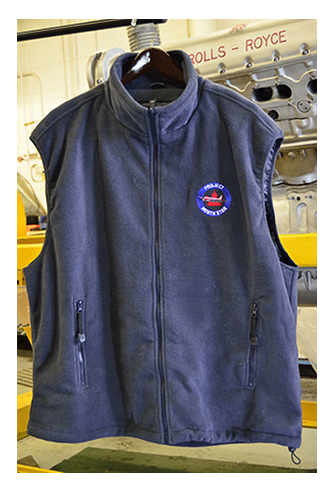
\includegraphics[scale=1.0]{fleece_YOW7578.eps}
%   %caption of the figure 
%   \caption*{\small \em PNSAC winter apparel}
%   %label of the figure, which has to correspond to \ref{}:
%   \label{fig:merchandise}
%\end{figure}

\begin{enumerate}
	\item "The Canadian North Star." This book and others referencing the North Star is available through Canavbooks ({\normalfont\color{blue}\texttt{\href{http://www.canavbooks.com}{www.canavbooks.com}}}).
	\item "Short on Silence" is an article on CASM's North Star, included in the February 2016 edition of the British publication {\normalfont\color{blue}\texttt{\href{http://www.flypast.com/}{Fly Past Magazine}}}.
	\item Models. There are only two metal models of the North Star left, and it is not presently intended to re-order. The models are for sale at CASM's gift shop.
\end{enumerate}



\begin{footnotesize}
    \raggedleft PNSAC\\
\end{footnotesize}

\begin{multicols}{2}

% End of text.

%%% Local Variables: 
%%% mode: latex
%%% TeX-master: main_document.tex
%%% End: 

 
% \end{article}

%\pagebreak


% Forthcoming events ................................................. %

%\begin{article}
%   
% Template PNSAC newsletter - Miscellany
% Language: Latex
\vspace{25mm}

\title{Calendar of Events}

\maketitle

\end{multicols}

\begin{tabbing}
%June 5, 2014     \hspace{50mm}\= Board of Directors' Meeting\\
%{\normalfont\color{red}May 02, 2015}   \hspace{50mm}\= 
%{\normalfont\color{red}Members' Quarterly Meeting}\\
May 26, 2016   \hspace{50mm}\= Board of Directors' Meeting\\ 
July 01, 2016  \> Canada Day\\
September 15, 2016   \> Board of Directors' Meeting\\
September 24, 2016 \> Annual General Meeting

\end{tabbing}

%\noindent \textbf{Note}: The next Quarterly meeting will be held in the boardroom of
%{\normalfont\color{blue}\texttt{\href{https://http://www.vintagewings.ca/}{Vintage
%      Wings of Canada }}} at 10:00 AM on April 12, 2014.  A hangar tour will follow the meeting. 

\begin{multicols}{2}

%%% Local Variables: 
%%% mode: latex
%%% TeX-master: main_document.tex
%%% End: 

 
%\end{article}
%
%\pagebreak


% Board members/contact info ......................................... %

\begin{article}
  
% Template PNSAC newsletter - Contact information
% Language: Latex

% Removes superscript from footnotes
\renewcommand\thefootnote{\relax}

% \renewcommand\thefootnote{\relax} 
%This is cheap and (moderately) cheerful, but it has some odd 
%properties. 
%If you want numbered footnotes again subsequently in your document, 
%you should say: 
%  \let\oldthefootnote\thefootnote 
%  \renewcommand\thefootnote{\relax} 
%  ... 
%  \let\thefootnote\oldthefootnote 
%  ... (footnotes are numbered again) 
%One of the endearing properties of this technique is that the 
%footnotes are counted even if their number isn't printed 

\title{Board and Officer's Contact Information}

\maketitle

\subsection{Board of Directors}
%\label{sec:misc_pnsac_executive}

%\begin{minipage}{\columnwidth}

\address{Richard Lodge\\
Director, President\\
\email{president@projectnorthstar.ca}}

\address{Neil Raynor\\
Director, Vice President}\\

\address{Garry Dupont\\
Director}\\

\address{Roger Button\\
Director, Corporate Secretary, NStar Chronicle Editor}\\

\address{Phil Chrysler\\
Director, Merchandise}\\



%\address{Bill Tate\\
%Director, Special Events}\\
%613-523-8817\\
%\email{billtate@bell.net}}


%\end{minipage}

%\columnbreak

%\begin{minipage}{\columnwidth}

\columnbreak  

\vspace{12pt}

\subsection{Other Officers}

\address{Bruce Gemmill\\
Membership Secretary\\
\email{membership@projectnorthstar.ca}}

\address{Paul Labranche\\
Treasurer\\
\email{treasurer@projectnorthstar.ca}}

%\end{minipage}




\subsection{Newsletter\protect\footnotetext{This newsletter is typeset using
    \LaTeX.  The style package used for the newsletter (PNSAC.sty) is
    a modification of GRASSnews.sty belonging to the Geographic
    Analysis Resources Support System (GRASS). The modification was
    made possible by kind permission of the Editor-in-Chief of
    GRASS-News.}}

\small\address{Editor: Roger Button\\
\small\email{editor@projectnorthstar.ca}}

\address{Typesetter: Drew Hodge}

%\end{multicols}

%\vspace{5mm}

%\hspace{-10mm}
%\setlength\fboxrule{2pt}%
%\framebox{%
%\begin{minipage}{1\columnwidth}%
%\begin{center}
%If you would like to contribute an article to the NStar Chronicle,
%please contact Bruce Grant at 
%\par\end{center}

%\begin{center}
%\email{r_b_grant@yahoo.ca} 
%\par\end{center}

%\begin{center}
%Your comments on the contents of this issue are also appreciated.
%\par\end{center}%
%\end{minipage}}

%\begin{multicols}{2}

%\address{PNSAC Newsletter postal and Web site addresses:}

\subsection{Association General Contact Information}

\address{PNSAC\\
P.O.Box 44005\\
Ottawa, ON\\
K1K 4P8}\\

\address{Web site:
{\normalfont\color{blue}\texttt{\url{http://www.projectnorthstar.ca}}}\\
	General enquiries:\email{info@projectnorthstar.ca}}

%\scriptsize\address{Web site:
{\normalfont\color{blue}\texttt{\url{http://www.projectnorthstar.ca}}}\\














%\begin{footnotesize}
%This newsletter is typeset using \LaTeX
%  \end{footnotesize}

%%% Local Variables: 
%%% mode: latex
%%% TeX-master: main_document.tex
%%% End:  
\end{article}


%\textit{All photos by Guy Poirier.}

\end{document}

% \begin{figure}[htbp]
%    \vspace{2em}
%    \centering
%    %name of the graphic, without the path AND in EPS format:
%    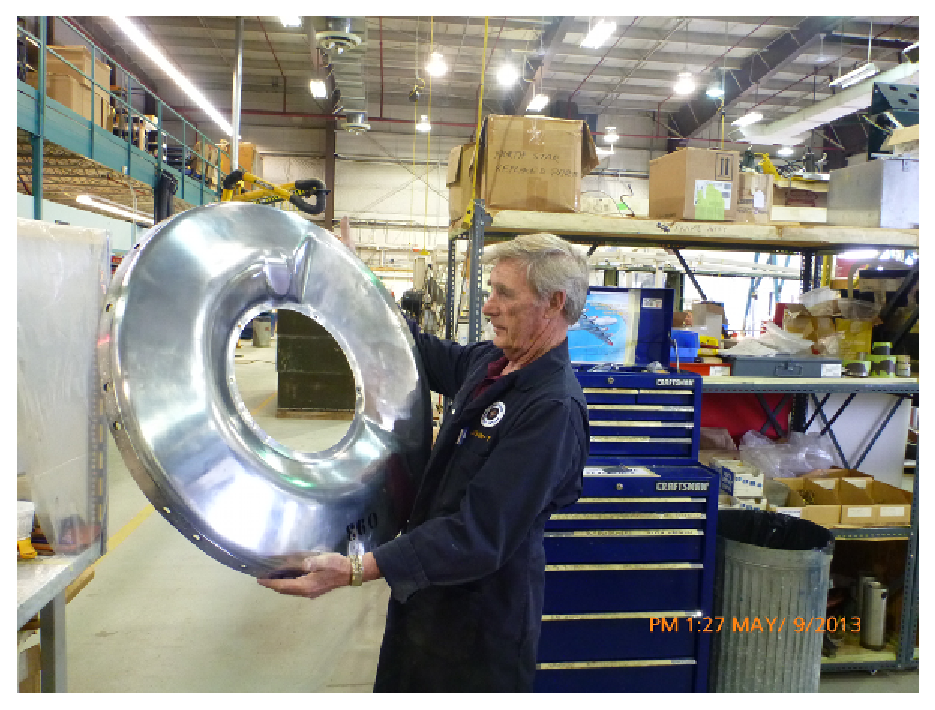
\includegraphics[scale=0.5]{engine3_prop_cowl.eps}
%    %caption of the figure 
%    \caption*{\small \em John Thibert with the propeller cowl for
%      engine nr 3.}
%    %label of the figure, which has to correspond to \ref{}:
%    \label{fig:engine3propcowl}
% \end{figure}

%%% Local Variables: 
%%% mode: latex
%%% TeX-master: main_document.tex
%%% End: 
